\documentclass[19pt,a4paper]{article}
\usepackage{xeCJK}
\usepackage{amsmath}
\setmainfont{STSong}
\usepackage{geometry}
\geometry{left=2.5cm,right=2.5cm,top=2.5cm,bottom=2.5cm}
\setlength{\parindent}{4em}
\usepackage{graphicx}
\title{算法作业6}
\author{孟妍廷2015202009}
\date{2017年10月30日}

\begin{document}
\maketitle
15.2-1\\
\indent 解: 依题意可得:
\begin{table}[h]
\centering
\begin{tabular*}{6cm}{lllllll}
\hline
$p_0$ & $p_1$ & $p_2$ & $p_3$ & $p_4$ & $p_5$ & $p_6$ \\
\hline
5 & 10 & 3 & 12 & 5 & 50 & 6 \\
\hline
\end{tabular*}
\end{table}\\
\indent 根据MATRIX-CHAIN-ORDER算法可得
$$m[i,i]=0,i=1....6$$
$$m[1,2]=m[1,1]+m[2,2]+p_0p_1p_2=150,k=1$$
$$m[2,3]=m[2,2]+m[3,3]+p_1p_2p_3=360,k=2$$
$$m[3,4]=m[3,3]+m[4,4]+p_2p_3p_4=180,k=3$$
$$m[4,5]=m[4,4]+m[5,5]+p_3p_4p_5=3000,k=4$$
$$m[5,6]=m[5,5]+m[6,6]+p_4p_5p_6=1500,k=5$$

$$m[1,3]=min\left\{
\begin{aligned}
m[1,1]+m[2,3]+p_0p_1p_3=0+360+5\times10\times12=960 \\
m[1,2]+m[3,3]+p_0p_2p_3=150+0+5\times3\times12=330 \ \ \ \star\\
\end{aligned}
\right.,k=2$$

$$m[2,4]=min\left\{
\begin{aligned}
m[2,2]+m[3,4]+p_1p_2p_4=0+180+10\times3\times5=330 \ \ \ \star \\
m[2,3]+m[4,4]+p_1p_3p_4=360+0+10\times12\times5=960 \\
\end{aligned}
\right.,k=2$$

$$m[3,5]=min\left\{
\begin{aligned}
m[3,3]+m[4,5]+p_2p_3p_5=0+3000+3\times12\times50=4800\\
m[3,4]+m[5,5]+p_2p_4p_5=180+0+3\times5\times50=930 \ \ \ \star\\
\end{aligned}
\right.,k=4$$

$$m[4,6]=min\left\{
\begin{aligned}
m[4,4]+m[5,6]+p_3p_4p_6=0+1500+12\times5\times6=1860 \ \ \ \star\\
m[4,5]+m[6,6]+p_3p_5p_6=3000+0+12\times50\times6=6600 \\
\end{aligned}
\right.,k=4$$

$$m[1,4]=min\left\{
\begin{aligned}
m[1,1]+m[2,4]+p_0p_1p_4=0+330+5\times10\times5=580\\
m[1,2]+m[3,4]+p_0p_2p_4=150+180+5\times3\times5=405 \ \ \ \star\\
m[1,3]+m[4,4]+p_0p_3p_4=330+0+5\times12\times5=630 \\
\end{aligned}
\right.,k=2$$

$$m[2,5]=min\left\{
\begin{aligned}
m[2,2]+m[3,5]+p_1p_2p_5=0+930+10\times3\times50=2430\ \ \ \star\\
m[2,3]+m[4,5]+p_1p_3p_5=360+3000+10\times12\times50=9360\\
m[2,4]+m[5,5]+p_1p_4p_5=330+0+10\times5\times50=2830\\
\end{aligned}
\right.,k=2$$

$$m[3,6]=min\left\{
\begin{aligned}
m[3,3]+m[4,6]+p_2p_3p_6=0+1860+3\times12\times6=2076\\
m[3,4]+m[5,6]+p_2p_4p_6=180+1500+3\times5\times6=1770\ \ \ \star\\
m[3,5]+m[6,6]+p_2p_5p_6=930+0+3\times50\times6=1830\\
\end{aligned}
\right.,k=4$$

$$m[1,5]=min\left\{
\begin{aligned}
m[1,1]+m[2,5]+p_0p_1p_5=0+2430+5\times10\times50=4930\\
m[1,2]+m[3,5]+p_0p_2p_5=150+930+5\times3\times50=1830\\
m[1,3]+m[4,5]+p_0p_3p_5=330+3000+5\times12\times50=6330\\
m[1,4]+m[5,5]+p_0p_4p_5=405+0+5\times5\times50=1655\ \ \ \star\\
\end{aligned}
\right.,k=4$$

$$m[2,6]=min\left\{
\begin{aligned}
m[2,2]+m[3,6]+p_1p_2p_6=0+1770+10\times3\times6=1950\ \ \ \star\\
m[2,3]+m[4,6]+p_1p_3p_6=360+1860+10\times12\times6=2940\\
m[2,4]+m[5,6]+p_1p_4p_6=330+1500+10\times5\times6=2130\\
m[2,5]+m[6,6]+p_1p_5p_6=2430+0+10\times50\times6=5430\\
\end{aligned}
\right.,k=2$$

$$m[1,6]=min\left\{
\begin{aligned}
m[1,1]+m[2,6]+p_0p_1p_6=0+1950+5\times10\times6=2250\\
m[1,2]+m[3,6]+p_0p_2p_6=150+1770+5\times3\times6=2010\ \ \ \star\\
m[1,3]+m[4,6]+p_0p_3p_6=330+1860+5\times12\times6=2550\\
m[1,4]+m[5,6]+p_0p_4p_6=405+1500+5\times5\times6=2055\\
m[1,5]+m[6,6]+p_0p_5p_6=1655+0+5\times50\times6=3155\\
\end{aligned}
\right.,k=2$$

\indent 可得m矩阵和s矩阵如图:
\begin{figure}[htbp]
 \centering
 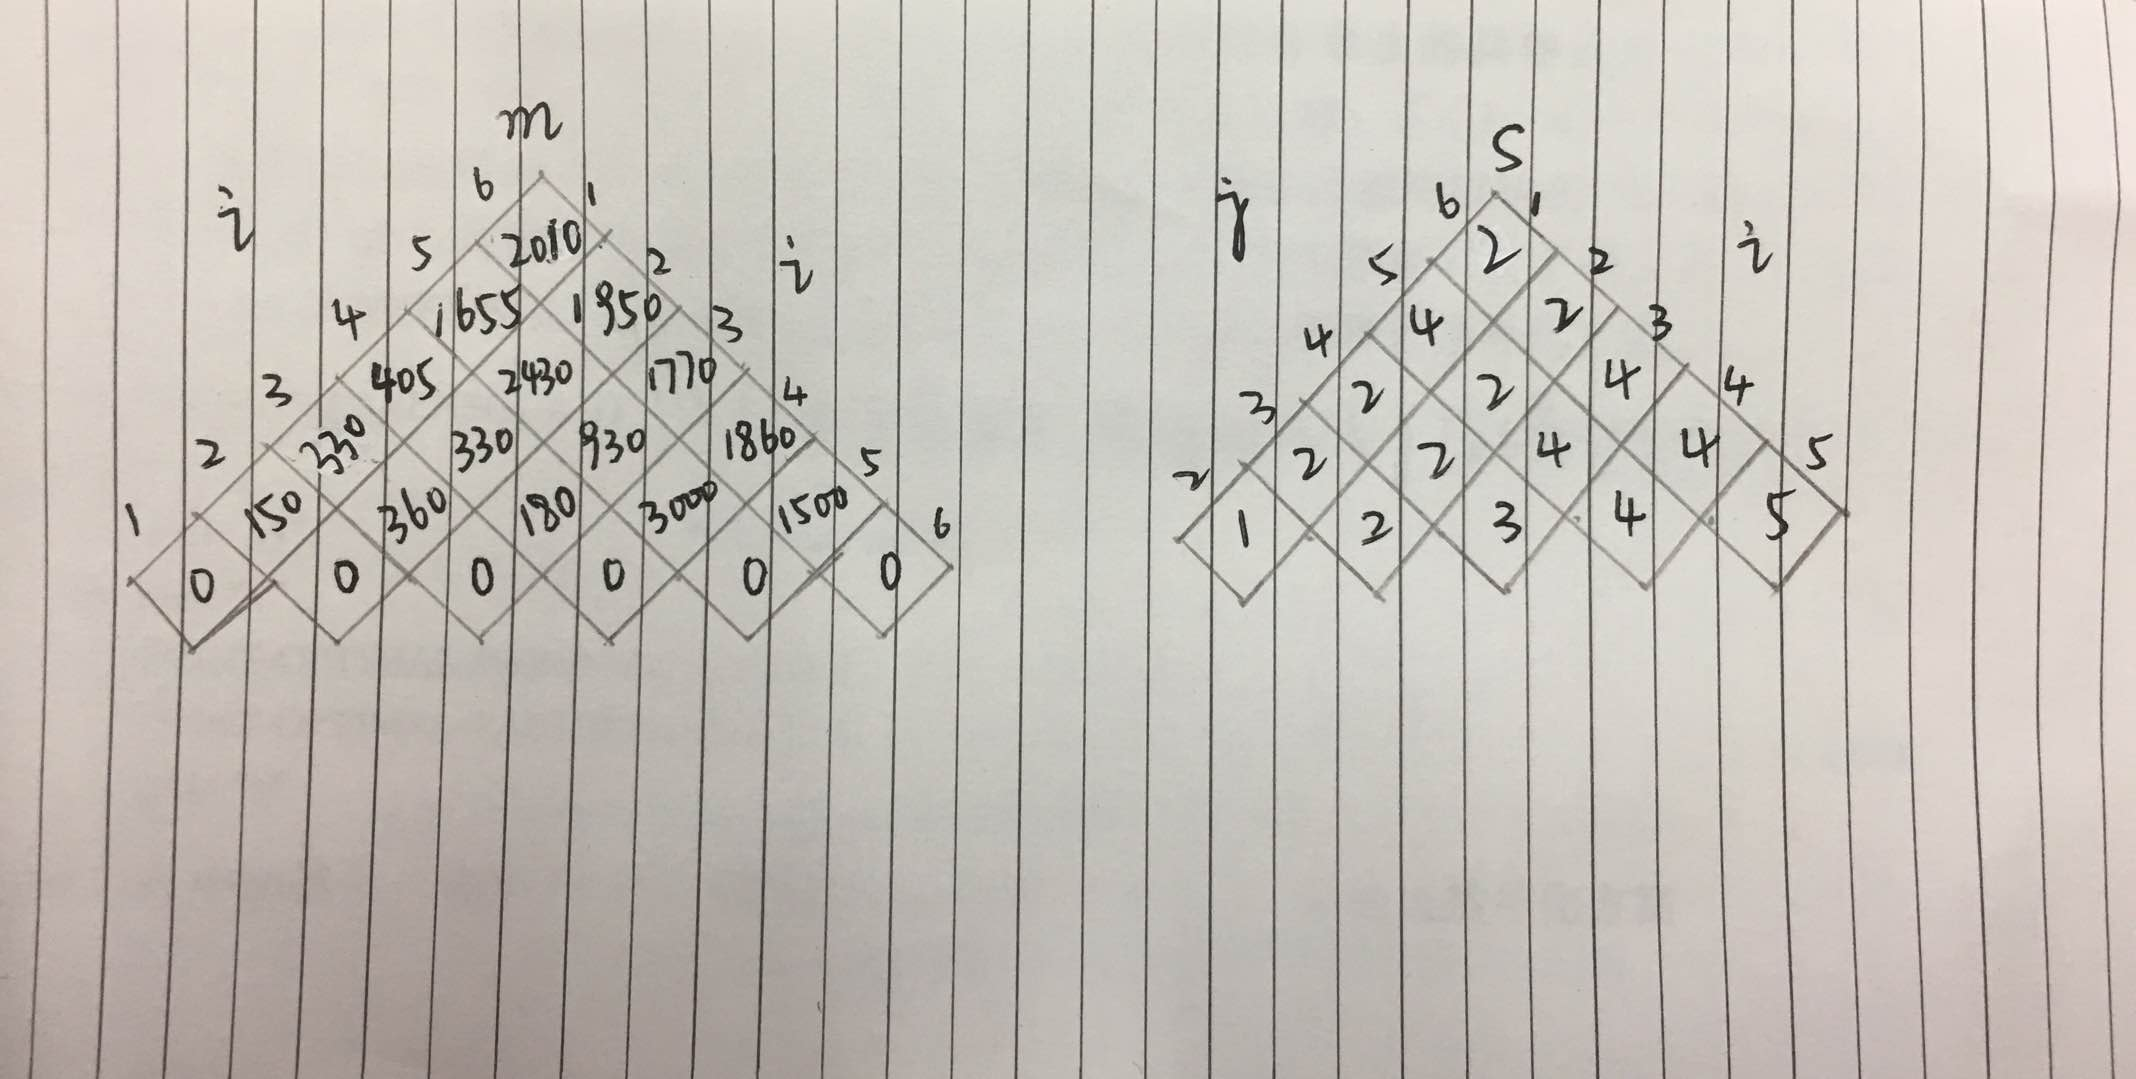
\includegraphics[scale=0.2]{h6.jpeg}
\end{figure}\\
\indent 根据PRINT-OPTIMAL-PARENS算法可得最优括号方案为$((A_1A_2)((A_3A_4)(A_5A_6)))$\\
\\
\indent 5.2\\
\indent 解:用动态规划求解:\\
\indent 由思考题讲解的分析可知,对于任意字符串,如果头和尾相同,那么它的最长回文子序列一\\
\indent 定是去头去尾之后的部分的最长回文子序列加上头和尾。如果头和尾不同,那么它的最长回\\
\indent 文子序列是去头部分和去尾部分的最长回文子序列中较长的一个。则可知:\\
\\
\indent $设字符串为s,f(i,j)表示s(i...j)的最长回文子序列\\
\indent 当i>j时,f(i,j)=0\\
\indent 当i=j,f(i,j)=1\\
\indent 当i<j时:\\
\indent f(i,j)=\left\{
\begin{aligned}
2+f(i+1,j-1),s[i]=s[j]\\
max\{f(i+1,j),f(i,j-1)\},s[i]\ne s[j]\\
\end{aligned}
\right.$\\
\\
\indent 则算法如下:\\
\indent $SOLUTION(s)\\
\indent \ \ \ \ let\ b[1....n,1...n],f[1...n,1...n]be\ new\ tables\\
\indent \ \ \ \ for\ i=1\ to n\\
\indent \ \ \ \ \ \ \ \ f[i,i]=1\\
\indent \ \ \ \ for\ i=n\ to\ 2\\
\indent \ \ \ \ \ \ \ \ for\ j=i-1\ to\ 1\\
\indent \ \ \ \ \ \ \ \ \ \ \ \ f[i,j]=0\\
\indent \ \ \ \ for\ i=n-1\ to\ 1\\
\indent \ \ \ \ \ \ \ \ for\ j=i+1\ to\ n\\
\indent \ \ \ \ \ \ \ \ \ \ \ \ if\ s[i]==s[j]\\
\indent \ \ \ \ \ \ \ \ \ \ \ \ \ \ \ \ f[i,j]=f[i+1,j-1]+2\\
\indent \ \ \ \ \ \ \ \ \ \ \ \ \ \ \ \ b[i,j]=\nwarrow\\
\indent \ \ \ \ \ \ \ \ \ \ \ \ elseif\ f[i+1,j] \ge f[i,j-1]\\
\indent \ \ \ \ \ \ \ \ \ \ \ \ \ \ \ \ f[i,j]=f[i+1,j]\\
\indent \ \ \ \ \ \ \ \ \ \ \ \ \ \ \ \ b[i,j]=\rightarrow\\
\indent \ \ \ \ \ \ \ \ \ \ \ \ else\ f[i,j]=f[i,j-1]\\
\indent \ \ \ \ \ \ \ \ \ \ \ \ \ \ \ b[i,j]=\uparrow\\
\indent \ \ \ \ return\ b\ and\ f$\\
\indent 时间复杂度为$O(n^2)$.\\
\indent $PRINT(b,s,i,j)\\
\indent \ \ \ \ if\ i<0\ or\ j<0\ or\ i>j\\
\indent \ \ \ \ \ \ \ \ return
\indent \ \ \ \ if\ b[i,j]=\nwarrow\\
\indent \ \ \ \ \ \ \ \ PRINT(b,s,i+1,j-1)\\
\indent \ \ \ \ \ \ \ \ print\ s_i,s_j\\
\indent \ \ \ \ elseif\ b[i,j]=\rightarrow\\
\indent \ \ \ \ \ \ \ \ PRINT(b,s,i+1,j)\\
\indent \ \ \ \ else\ PRINT(b,s,i,j-1)\\$
\indent 时间复杂度为$O(2n)$.\\
\\
\indent 15-4(整齐打印)\\
\indent 解:利用动态规划,在考虑第i到第j个词时,认为前i-1个词已经实现整齐打印,初始状态为0\\
\indent 算法如下:\\
\indent $SOLUTION(s)\\
\indent \quad fist[1...n]={0}//记录排好后,每一行首单词下标\\
\indent \quad a[1...n,1...n]//记录第i个数到第j个数若在一行的额外空格符数量\\
\indent \quad b[1...n,1...n]//记录排好后第i个数到第j个数的额外空格符数量\\\
\indent \quad rest[0...n]=\infty//记录排到每一个状态时的额外空格符数量\\
\indent \quad for\ i=1\ to\ n\\
\indent \quad \quad a[i,i]=M-l_i\\
\indent \quad \quad for\ j=i+1\ to\ n\\
\indent \quad \quad \quad a[i,j]=a[i,j-1]-l_j\\
\indent \quad for\ i=1\ to\ n\\
\indent \quad \quad for\ j=i\ to\ n\\
\indent \quad \quad \quad if\ a[i,j]<0//说明不在一行\\
\indent \quad \quad \quad \quad b[i,j]=\infty\\
\indent \quad \quad \quad elseif\ j==n//最后一行\\
\indent \quad \quad \quad \quad b[i,j]=0\\
\indent \quad \quad \quad else\ b[i,j]=a[i,j]^3\\
\indent \quad rest[0]=0//初始状态为0\\
\indent \quad for\ j=1\ to\ n\\
\indent \quad \quad for\ i=1\ to\ j\\
\indent \quad \quad \quad if\ rest[i-1]\ne\infty\ and\ b[i,j]\ne\infty\ and\ rest[i-1]+b[i,j]>rest[i]\\
\indent \quad \quad \quad \quad rest[j]=rest[i-1]+b[i,j]//i到j为一行\\
\indent \quad \quad \quad \quad fist[j]=i//首元素\\$
\indent 时间复杂度为$O(n^2)$,空间复杂度为O(2n).\\
\indent $PRINT(s,first,j)\\
\indent \quad i=first[j]//j所在行的首元素下标\\
\indent \quad if\ i=1\\
\indent \quad \quad return\\
\indent \quad PRINT(s,first,i-1)//递归\\
\indent \quad for\ k=i\ to\ j\\
\indent \quad \quad print(s_k)\\$
\indent 时间复杂度为O(n),空间复杂度为O(1).







\end{document}
